\documentclass[11pt]{report}
\usepackage{amsmath,amssymb,geometry,graphicx,hyperref}
\usepackage{listings} % for source code
\lstset{showstringspaces=false}
%%%%%%%%%%%%%%%%%%%%%%%%%%%%%%%%%%%%%%%%%%%%%%%%
% with 11 point font, 1.5 line spacing, single-sided pages
\setlength{\parskip}{0.5\baselineskip}
\usepackage[doublespacing]{setspace} % don't use onehalfspacing
\usepackage{titlesec}
\titlespacing*{\chapter}{0pt}{-50pt}{20pt}
\titleformat{\chapter}[hang]{\normalfont\huge\bfseries}{\thechapter}{1em}{} 
\newcommand{\cmd}[1]{\texttt{\textbackslash{}#1}}
\newcommand{\unnumberedchapter}[1]{\chapter*{#1}\addcontentsline{toc}{chapter}{#1}}  
\let\tempit\itemize \let\tempeit\enditemize \renewenvironment{itemize}{\vspace{-1em}\tempit\addtolength{\itemsep}{-0.5\baselineskip}}{\tempeit} % Changes itemize spacing
\let\tempen\enumerate \let\tempeen\endenumerate \renewenvironment{enumerate}{\vspace{-1em}\tempen\addtolength{\itemsep}{-0.5\baselineskip}}{\tempeen} % Changes enumerate spacing
%%%%%%%%%%%%%%%%%%%%%%%%%%%%%%%%%%%%%%%%%%%%%%%%

\title{Project Title} 
\author{Author Name}
\date{September 201x}

\begin{document} 
\begingroup \let\newpage\relax \maketitle \endgroup % This temporarily redefines newpage so that there is no page break after the maketitle.

\vspace*{\stretch{1}}
\begin{center}\bf
    Dissertation submitted in partial fulfillment for the degree of \\
    Master of Science in \textit{(insert your degree title)} \\[1em]
    
    Computing Science and Mathematics \\
    University of Stirling
\end{center}


\unnumberedchapter{Abstract}
\pagenumbering{roman}

Summary of the dissertation \textbf{\textit{within one page}}. 

This template starts the page numbering at the foot of this page. While you are printing drafts, you might find it useful to add the printing date and time into the footer -- to help you, and your supervisor, tell which version is most current.

\textbf{Note: You are required to submit one extra copy of your title page and Abstract.}

It is suggested that the abstract be structured as follows:
\begin{itemize}
	\item Problem: What you tackled, and why this needed a solution
	\item Objectives: What you set out to achieve, and how this addressed the problem
	\item Methodology: How you went about solving the problem
	\item Achievements: What you managed to achieve, and how far it meets your objectives.
\end{itemize}


\unnumberedchapter{Attestation}

I understand the nature of plagiarism, and I am aware of the University?s policy on this.

I certify that this dissertation reports original work by me during my University project except for the following (\textit{adjust according to the circumstances}):
\begin{itemize}
    \item The technology review in Section 2.5 was largely taken from [17].
    \item The code discussed in Section 3.1 was created by Acme Corporation (\url{www.acme-corp.com/JavaExpert}) and was used in accordance with the licence supplied.
    \item The code discussed in Section 3.5 was written by my supervisor.
    \item The code discussed in Section 4.2 was developed by me during a vacation placement with the collaborating company. In addition, this used ideas I had already developed in my own time.
\end{itemize}

\vspace*{\stretch{1}}

\textbf{Signature:} \hspace{\stretch{1}}%
\textit{(you must delete this, then sign and date this page)} % In TeX, delete this line entirely.
\hspace{\stretch{1}} \textbf{Date}


\unnumberedchapter{Acknowledgements}

Acknowledge anyone who has helped you in your work such as your supervisor, technical support staff, fellow students or external organisations. Acknowledge the source of any work that is not your own.


\unnumberedchapter{How to Create Table of Contents and List of Figures}

The table of contents on the following page is automatically generated from the \cmd{part}, \cmd{section}, \cmd{subsection}, etc., commands in the \texttt{.tex} file. Depending on your configuration, you may have to typeset your document twice in order to update this section (the first typesetting will create a \texttt{.toc} file, which is then used during the second typesetting).

Similarly you can automatically generate a list of figures from the \cmd{begin\{figure\}} and \cmd{end\{figure\}} commands in this document. Again, you may need to typeset your document twice in order for this list to update.

In your document, remove this entire section and only leave the lines
\begin{quote}
	\cmd{tableofcontents} \\
	\cmd{listoffigures}
\end{quote}
These automatically begin new pages that look like Chapters in the finished pdf.

\begingroup
\singlespacing
\tableofcontents
\endgroup

\begingroup
\singlespacing
\listoffigures
\endgroup

\chapter{Introduction}
\pagenumbering{arabic}
For editorial consistency, it is important to use \LaTeX{} formatting properly. To use italics, replace the dots in \cmd{textit\{\ldots\}} with the text you would like to be italicized. To make text bold, use \cmd{textbf}.

Chapters are entered using the \cmd{chapter} command. For example, this chapter begins with \cmd{chapter\{Introduction\}} in the \texttt{.tex} file. The chapter command automatically moves to the start of a new page and supplies the next chapter number. The first paragraph after a heading automatically will have no indent on the first line. In the \texttt{.tex} file, it does not matter whether you leave a blank line after the \cmd{chapter} command or not -- the typeset pdf will have it anyway.

The remaining paragraphs will have an indent.

In general, use the default spacing that headings and paragraphs give you. Avoid using new-lines or spaces to format text. If you need to use quotes, preferably use single curly quotes `\ldots'. In the \texttt{.tex} file, the opening quote is typed as a grave accent (\`{}) and the closing quote is typed as an apostrophe ($^\prime\,$). If you wish to emphasise something, usually use italic font.

\textbf{Remember to save frequently while you are working!}

\section{Background and Context}

Give the background to your project and context of what you have done. Sections within a chapter are entered using the \cmd{section} command, which automatically supplies the next section number.

\section{Scope and Objectives} \label{objectives sec}
Define the scope and objectives of your project.

\section{Achievements}
Summarise what you have achieved.

\section{Overview of Dissertation}
Briefly overview the contents of what follows in the dissertation.

\chapter{State-of-the-Art}
Summarise current knowledge and what others have done in the various topics of your dissertation -- in the application area and in the various technologies that you might have used or did use. Write for someone familiar with computing, but not necessarily expert in the particular topics of your project. Give references to other work by using cross-references to entries in the References section, like this [2].

\chapter{Technical Chapters (change this to something appropriate)}
\textbf{Note: This part of the dissertation will normally be expanded to be a \textit{series of chapters}.}

The technical body of the dissertation consists of a number of chapters (just one here, but there will usually be more).  Follow a logical structure in how you present your work.  This will usually be the phases of the software development cycle, the modules of your system, etc. \textbf{\textit{However, please do not write your dissertation to read like a diary.}}

Include a chapter demonstrating what you have achieved and how your system is used in practice -- for example showing a typical session as a series of pasted in screen shots, with an accompanying commentary.

You \textbf{\textit{should}} also include a chapter explaining how you obtained feedback from your ``customer'' or potential users of your system, what feedback you actually obtained, and your analysis and comments.

\section{First Section}
Subdivide your text into sections, using the \cmd{section} command.

\subsection{First Subsection}
If necessary, also use subsections. Subsections are entered using the \cmd{subsection} command (all these heading styles are self-numbering).

%\subsubsection{First Subsubsection}
%If you really need subsubsections, enter these using the \cmd{subsubsection} command. Note that subsubsections in \TeX{} do not display numbers or appear in the Table of Contents (they just show a bold header on its own line).

\subsection{Second Subsection}
And, as required, more subsections.

\section{Bulleted and Numbered Lists}
Note: This section begins with the code \texttt{\textbackslash{}section\{Bulleted and Numbered Lists\}} in the~\texttt{.tex} file.

Bulleted or numbered lists are entered using the \texttt{itemize} and \texttt{enumerate} environments, respectively. An \textbf{environment} in \LaTeX{} is a block of code in between a \cmd{begin} and \cmd{end} command. For example, the code
\begin{quote}\tt
	\textbackslash{}begin\{itemize\} \\[-0.5em]
	\hspace*{2em}\textbackslash{}item Up \\[-0.5em]
	\hspace*{2em}\textbackslash{}item Down \\[-0.5em]
	\hspace*{2em}\textbackslash{}item Left \\[-0.5em]
	\hspace*{2em}\textbackslash{}item Right \\[-0.5em]
	\textbackslash{}end\{itemize\}
\end{quote}
would produce the following list:
\begin{itemize} \item Up \item Down \item Left \item Right \end{itemize}
The indentation is not necessary (the pdf will look the same even it the \texttt{.tex} file does not use indents), but it helps make the code easier to read.

If the \texttt{enumerate} environment is used instead, the bullets are replaced by numbers. For example, the code
\begin{quote}\tt
	\textbackslash{}begin\{enumerate\} \\[-0.5em]
	\hspace*{2em}\textbackslash{}item Up \\[-0.5em]
	\hspace*{2em}\textbackslash{}item Down \\[-0.5em]
	\hspace*{2em}\textbackslash{}item Left \\[-0.5em]
	\hspace*{2em}\textbackslash{}item Right \\[-0.5em]
	\textbackslash{}end\{enumerate\}
\end{quote}
produces the list
\begin{enumerate} \item Up \item Down \item Left \item Right \end{enumerate}

\section{Figures and Captions}
As an example of a figure, consider Figure \ref{mylovelydiagram}. Captions are entered using the \texttt{figure} environment (read the previous section for information about environments in general). The code
\begin{quote}\tt
	\textbackslash{}begin\{figure\}[h] \\[-0.5em]
	\hspace*{2em}\textbackslash{}center\textbackslash{}includegraphics[width=12cm]\{image.jpg\} \\[-0.5em]
	\hspace*{2em}\textbackslash{}caption\{Highly Technical Diagram\} \\[-0.5em]
	\hspace*{2em}\textbackslash{}label\{mylovelydiagram\} \\[-0.5em]
	\textbackslash{}end\{figure\}
\end{quote}
will produce the following figure \textbf{if the file \textit{image.jpg} is in the same folder as your \texttt{.tex} file}.
\begin{figure}[h]
	\center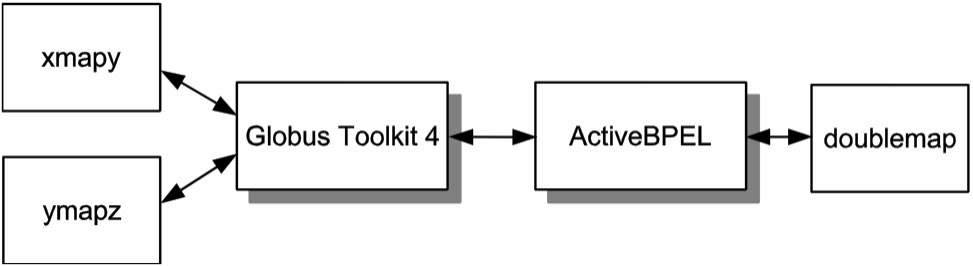
\includegraphics[width=12cm]{image.jpg}
	\caption{Highly Technical Diagram}
	\label{mylovelydiagram}
\end{figure}

The \texttt{[h]} direction after the beginning of the environment causes the figure to be placed ``here'' in the text (at least approximately -- sometimes \TeX{} will move the figure slightly if the spacing does not work well in exactly the given location). For large figures, use \texttt{[t]} or~\texttt{[b]} instead to place the figure at the top or bottom of a page. You can also leave off the \texttt{[h]} entirely to have \TeX{} make its best guess for where the figure should go.

The \cmd{includegraphics} command puts an image file from your computer into your finished pdf. \textbf{If there is no file with the given name in the folder with your \texttt{.tex} file, your document will not compile at all.} The bracket text \texttt{[width=12cm]} is optional; without it, \TeX{} will use the normal size of the image. Sometimes this will be far too large, so it is a good idea to specify a width directly.

Figures have automatic numbering, and it is possible to make cross-references to figures. The code \cmd{ref\{mylovelydiagram\}} will create a link ``\ref{mylovelydiagram}'' in the text with the number of that figure. You can change the text ``mylovelydiagram'' to be anything you want -- it never appears in the final pdf.

\section{Source Code}

To include programming source code in your document, use the \texttt{lstlisting} environment. The \LaTeX{} code
\begin{quote}\tt
	\textbackslash{}begin\{lstlisting\}[language=Python, frame=single] \\[-0.5em]
    \hspace*{2em}def factorial(n): \\[-0.5em]
    \hspace*{4em}if n == 0: return 1 \\[-0.5em]
    \hspace*{4em}else: return n * factorial(n-1) \\[-0.5em]
    \textbackslash{}end\{lstlisting\}
\end{quote}
produces the following in the pdf: \\
\begin{lstlisting}[language=Python, frame=single, basicstyle=\ttfamily]
def factorial(n):
	if n == 0: return 1
	else: return n * factorial(n-1)
\end{lstlisting}
You can change \texttt{language=Python} to \texttt{language=Java}, etc., for different programming languages. The \texttt{frame=single} can be removed if you do not want the border around your code snippet. See \url{https://en.wikibooks.org/wiki/LaTeX/Source_Code_Listings} for syntax coloring and other options.


\chapter{Conclusion}

\section{Summary}
Summarise what you have achieved.

\section{Evaluation}
Stand back and evaluate what you have achieved and how well you have met the objectives. Evaluate your achievements against your objectives in section \ref{objectives sec}. Demonstrate that you have tackled the project in a professional manner. 

The previous paragraph demonstrates the use of automatic cross-references:  The ``1.2'' is a \textit{cross-reference} to the text in a numbered item of the document; you do not type it as \texttt{1.2} but by using the \cmd{ref} command. The number that appears here will change automatically if the number on the referred-to section is altered, for example, if a chapter or section is added or deleted before it. Cross-references to section are entered with the \cmd{ref} command just like for figures. The \TeX{} code above reads
\begin{quote}\tt
	Evaluate your achievements against your objectives \\[-0.5em]
	in section \textbackslash{}ref\{objectives sec\}.
\end{quote}
For this to work, the code for the text on page \pageref{objectives sec} must read
\begin{quote}\tt
	\textbackslash{}section\{Scope and Objectives\} \textbackslash{}label\{objectives sec\}
\end{quote}
As with figure labels, the text inside of \cmd{label} and \cmd{ref} never appears in the final pdf; you can make it whatever you want as long as you use the same text in each to complete the reference.

\section{Future Work}
Explain any limitations in your results and how things might be improved. Discuss how your work might be developed further.  Reflect on your results in isolation and in relation to what others have achieved in the same field. This self-analysis is particularly important.  You should give a critical evaluation of what went well, and what might be improved.


\unnumberedchapter{How to Create a References section}

Although it looks like a Chapter in the finished pdf, the References section is created using an environment called \texttt{thebibliography} rather than a \cmd{chapter} command. Each item in your bibliography should be typed in the \texttt{.tex} file as its own paragraph that begins with the \cmd{bibitem} command. The first reference below is typed as
\begin{quote}\tt
	\textbackslash{}bibitem\{GW\} Greene, D. and Williams, P. C. \textbackslash{}textit\{Linear Accelerators for Radiation Therapy\}, Second Edition. IOP Publishing Ltd., Bristol and Philadelphia, 1997.
\end{quote}
Books~\cite{GW}, standards~\cite{ISO}, reports~\cite{JA}, journal articles~\cite{Turner}, conference papers~\cite{JT}, and web pages~\cite{Stirling} are conventionally presented in slightly different ways. Put urls in the~\cmd{url} command to give them fixed-width formatting and an automatic link.

To cite an item from your bibliography in the text, use the \cmd{cite} command, which essentially pairs with \cmd{bibitem} the same way that \cmd{ref} pairs with \cmd{label}. For example, the previous paragraph begins
\begin{quote}\tt
	Books \textbackslash{}cite\{GW\}, standards ...
\end{quote}

\begin{thebibliography}{99999}

\bibitem{GW} Greene, D. and Williams, P. C. \textit{Linear Accelerators for Radiation Therapy}, Second Edition. IOP Publishing Ltd., Bristol and Philadelphia, 1997.

\bibitem{ISO} ISO. \textit{Language Of Temporal Ordering Specification}, ISO 8807, International Organization for Standardization, Geneva, 1989.

\bibitem{JA} Jacobson, J. and Andersen, O., editors. \textit{Software Controlled Medical Devices}. SP Report 1997:11, Swedish National Testing and Research Institute, Sweden, 1997.

\bibitem{Turner} Turner, K. J. The Rules for Sailing Races on PDAs, \textit{J. Navigation}, 23(5):114-240, May 2002.

\bibitem{JT} Ji, H. and Turner, K. J. Specification and Verification of Synchronous Hardware using LOTOS. In Wu, J. Chanson, S. T. Gao, Q. editors, \textit{Proc.~Formal Methods for Protocol Engineering and Distributed Systems} (FORTE XII/PSTV XIX), pages 295-312, Kluwer Academic Publishers, London, UK, October 1999.

\bibitem{Stirling} University of Stirling. Computing Science and Mathematics Research Home Page, \url{http://www.cs.stir.ac.uk/research}, April 2002.

\end{thebibliography}

\unnumberedchapter{Appendix 1}
You may have one or more appendices containing detail, bulky or reference material that is relevant though supplementary to the main text: perhaps additional specifications, tables or diagrams that would distract the reader if placed in the main part of the dissertation. Make sure that you place appropriate cross-references in the main text to direct the reader to the relevant appendices.

\textit{Note that you should \textbf{\large not} include your program listings as an appendix or appendices.} You should submit one copy of such bulky text as a separate item, perhaps on a disk.

\unnumberedchapter{Appendix 2 -- User guide}
If you produced software that is intended for others to use, or that others may wish to extend/improve, then a user guide and an installation guide appendices are \textbf{\textit{essential}}.

\unnumberedchapter{Appendix 3 -- Installation guide}
If you produced software that is intended for others to use, or that others may wish to extend/improve, then a user guide and an installation guide appendices are \textbf{\textit{essential}}.


\end{document}